\documentclass[1p]{elsarticle_modified}
%\bibliographystyle{elsarticle-num}

%\usepackage[colorlinks]{hyperref}
%\usepackage{abbrmath_seonhwa} %\Abb, \Ascr, \Acal ,\Abf, \Afrak
\usepackage{amsfonts}
\usepackage{amssymb}
\usepackage{amsmath}
\usepackage{amsthm}
\usepackage{scalefnt}
\usepackage{amsbsy}
\usepackage{kotex}
\usepackage{caption}
\usepackage{subfig}
\usepackage{color}
\usepackage{graphicx}
\usepackage{xcolor} %% white, black, red, green, blue, cyan, magenta, yellow
\usepackage{float}
\usepackage{setspace}
\usepackage{hyperref}

\usepackage{tikz}
\usetikzlibrary{arrows}

\usepackage{multirow}
\usepackage{array} % fixed length table
\usepackage{hhline}

%%%%%%%%%%%%%%%%%%%%%
\makeatletter
\renewcommand*\env@matrix[1][\arraystretch]{%
	\edef\arraystretch{#1}%
	\hskip -\arraycolsep
	\let\@ifnextchar\new@ifnextchar
	\array{*\c@MaxMatrixCols c}}
\makeatother %https://tex.stackexchange.com/questions/14071/how-can-i-increase-the-line-spacing-in-a-matrix
%%%%%%%%%%%%%%%

\usepackage[normalem]{ulem}

\newcommand{\msout}[1]{\ifmmode\text{\sout{\ensuremath{#1}}}\else\sout{#1}\fi}
%SOURCE: \msout is \stkout macro in https://tex.stackexchange.com/questions/20609/strikeout-in-math-mode

\newcommand{\cancel}[1]{
	\ifmmode
	{\color{red}\msout{#1}}
	\else
	{\color{red}\sout{#1}}
	\fi
}

\newcommand{\add}[1]{
	{\color{blue}\uwave{#1}}
}

\newcommand{\replace}[2]{
	\ifmmode
	{\color{red}\msout{#1}}{\color{blue}\uwave{#2}}
	\else
	{\color{red}\sout{#1}}{\color{blue}\uwave{#2}}
	\fi
}

\newcommand{\Sol}{\mathcal{S}} %segment
\newcommand{\D}{D} %diagram
\newcommand{\A}{\mathcal{A}} %arc


%%%%%%%%%%%%%%%%%%%%%%%%%%%%%5 test

\def\sl{\operatorname{\textup{SL}}(2,\Cbb)}
\def\psl{\operatorname{\textup{PSL}}(2,\Cbb)}
\def\quan{\mkern 1mu \triangleright \mkern 1mu}

\theoremstyle{definition}
\newtheorem{thm}{Theorem}[section]
\newtheorem{prop}[thm]{Proposition}
\newtheorem{lem}[thm]{Lemma}
\newtheorem{ques}[thm]{Question}
\newtheorem{cor}[thm]{Corollary}
\newtheorem{defn}[thm]{Definition}
\newtheorem{exam}[thm]{Example}
\newtheorem{rmk}[thm]{Remark}
\newtheorem{alg}[thm]{Algorithm}

\newcommand{\I}{\sqrt{-1}}
\begin{document}

%\begin{frontmatter}
%
%\title{Boundary parabolic representations of knots up to 8 crossings}
%
%%% Group authors per affiliation:
%\author{Yunhi Cho} 
%\address{Department of Mathematics, University of Seoul, Seoul, Korea}
%\ead{yhcho@uos.ac.kr}
%
%
%\author{Seonhwa Kim} %\fnref{s_kim}}
%\address{Center for Geometry and Physics, Institute for Basic Science, Pohang, 37673, Korea}
%\ead{ryeona17@ibs.re.kr}
%
%\author{Hyuk Kim}
%\address{Department of Mathematical Sciences, Seoul National University, Seoul 08826, Korea}
%\ead{hyukkim@snu.ac.kr}
%
%\author{Seokbeom Yoon}
%\address{Department of Mathematical Sciences, Seoul National University, Seoul, 08826,  Korea}
%\ead{sbyoon15@snu.ac.kr}
%
%\begin{abstract}
%We find all boundary parabolic representation of knots up to 8 crossings.
%
%\end{abstract}
%\begin{keyword}
%    \MSC[2010] 57M25 
%\end{keyword}
%
%\end{frontmatter}

%\linenumbers
%\tableofcontents
%
\newcommand\colored[1]{\textcolor{white}{\rule[-0.35ex]{0.8em}{1.4ex}}\kern-0.8em\color{red} #1}%
%\newcommand\colored[1]{\textcolor{white}{ #1}\kern-2.17ex	\textcolor{white}{ #1}\kern-1.81ex	\textcolor{white}{ #1}\kern-2.15ex\color{red}#1	}

{\Large $\underline{11n_{137}~(K11n_{137})}$}

\setlength{\tabcolsep}{10pt}
\renewcommand{\arraystretch}{1.6}
\vspace{1cm}\begin{tabular}{m{100pt}>{\centering\arraybackslash}m{274pt}}
\multirow{5}{120pt}{
	\centering
	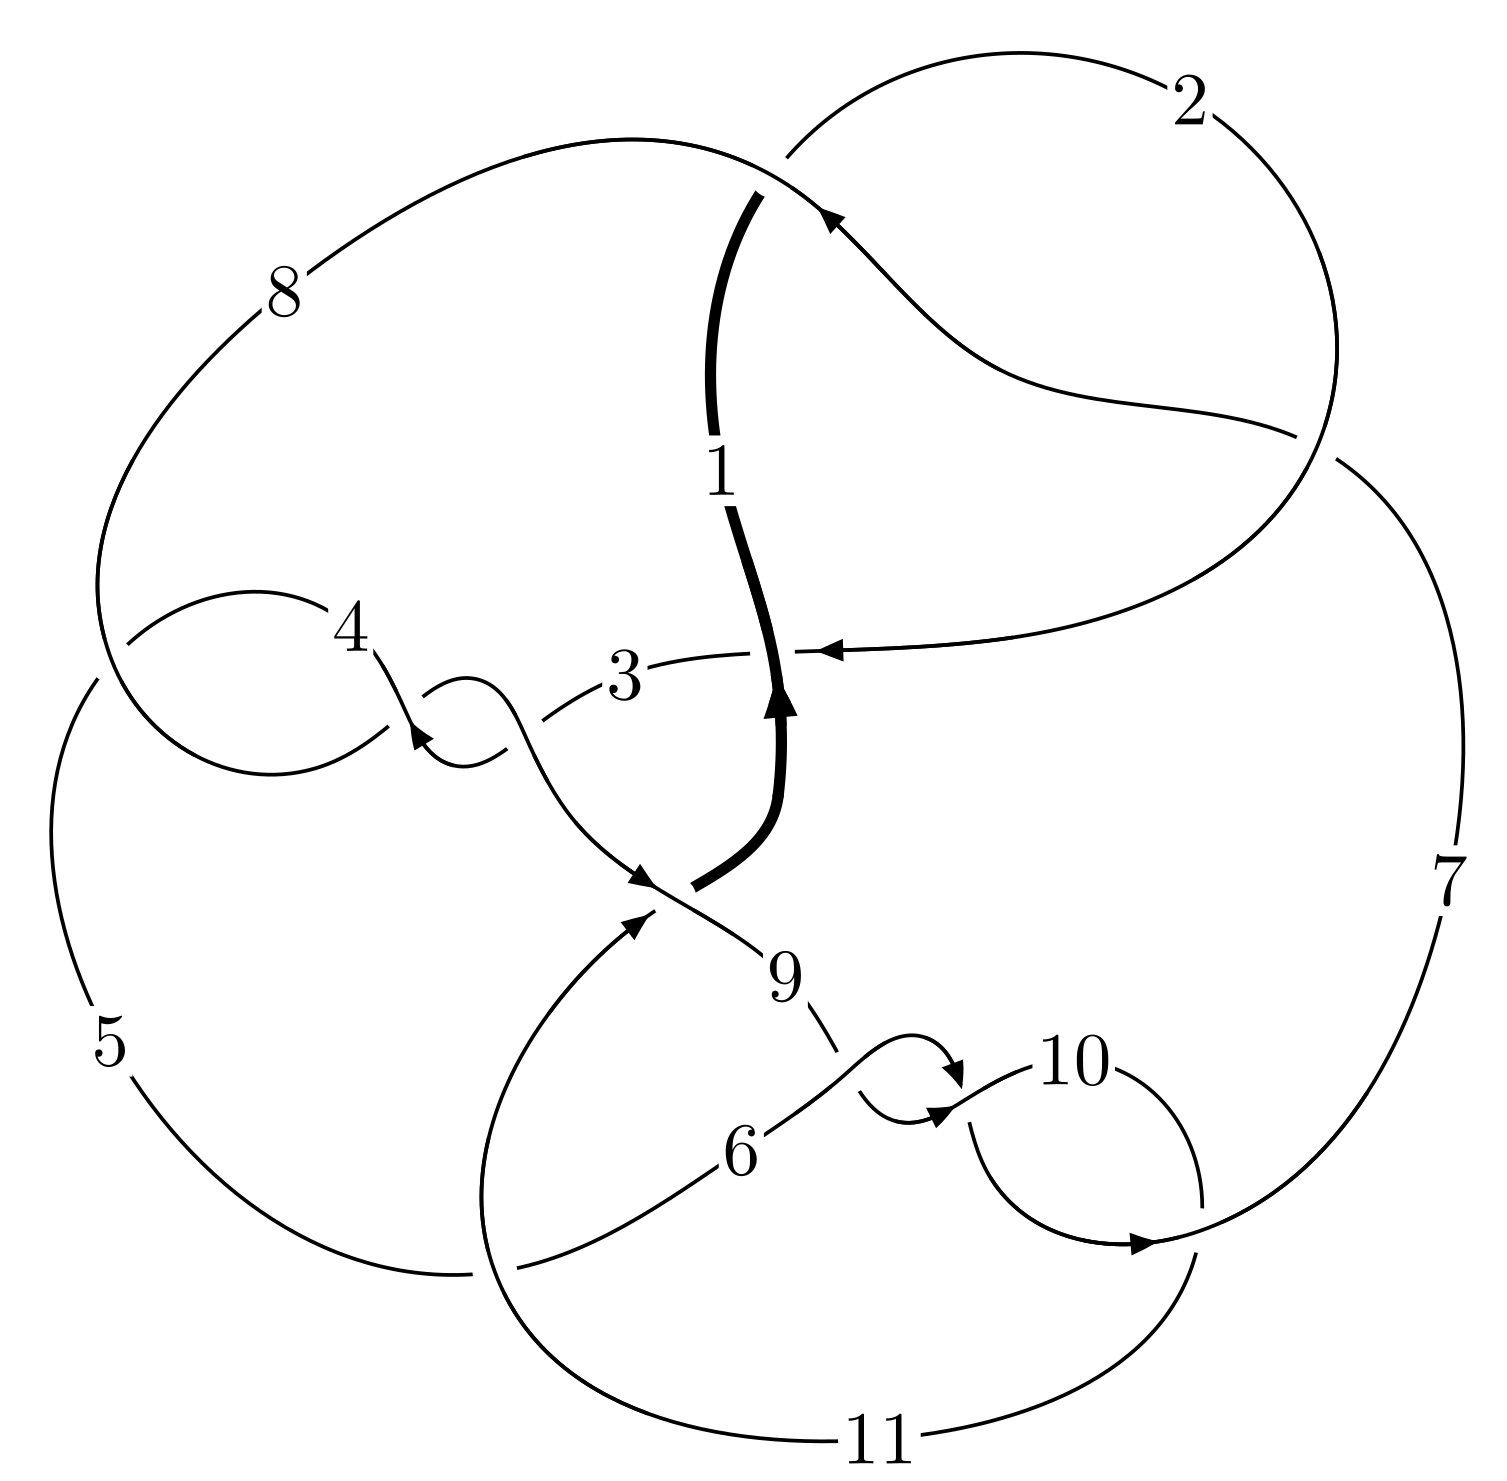
\includegraphics[width=112pt]{../../../GIT/diagram.site/Diagrams/png/753_11n_137.png}\\
\ \ \ A knot diagram\footnotemark}&
\allowdisplaybreaks
\textbf{Linearized knot diagam} \\
\cline{2-2}
 &
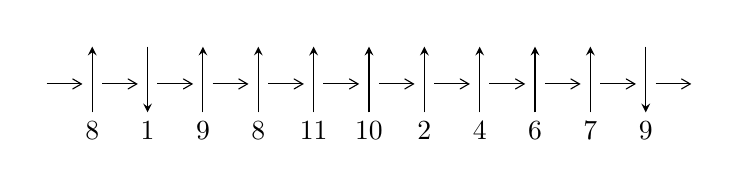
\begin{tikzpicture}[x=20pt, y=17pt]
	% nodes
	\node (C0) at (0, 0) {};
	\node (C1) at (1, 0) {};
	\node (C1U) at (1, +1) {};
	\node (C1D) at (1, -1) {8};

	\node (C2) at (2, 0) {};
	\node (C2U) at (2, +1) {};
	\node (C2D) at (2, -1) {1};

	\node (C3) at (3, 0) {};
	\node (C3U) at (3, +1) {};
	\node (C3D) at (3, -1) {9};

	\node (C4) at (4, 0) {};
	\node (C4U) at (4, +1) {};
	\node (C4D) at (4, -1) {8};

	\node (C5) at (5, 0) {};
	\node (C5U) at (5, +1) {};
	\node (C5D) at (5, -1) {11};

	\node (C6) at (6, 0) {};
	\node (C6U) at (6, +1) {};
	\node (C6D) at (6, -1) {10};

	\node (C7) at (7, 0) {};
	\node (C7U) at (7, +1) {};
	\node (C7D) at (7, -1) {2};

	\node (C8) at (8, 0) {};
	\node (C8U) at (8, +1) {};
	\node (C8D) at (8, -1) {4};

	\node (C9) at (9, 0) {};
	\node (C9U) at (9, +1) {};
	\node (C9D) at (9, -1) {6};

	\node (C10) at (10, 0) {};
	\node (C10U) at (10, +1) {};
	\node (C10D) at (10, -1) {7};

	\node (C11) at (11, 0) {};
	\node (C11U) at (11, +1) {};
	\node (C11D) at (11, -1) {9};
	\node (C12) at (12, 0) {};

	% arrows
	\draw[->,>={angle 60}]
	(C0) edge (C1) (C1) edge (C2) (C2) edge (C3) (C3) edge (C4) (C4) edge (C5) (C5) edge (C6) (C6) edge (C7) (C7) edge (C8) (C8) edge (C9) (C9) edge (C10) (C10) edge (C11) (C11) edge (C12) ;	\draw[->,>=stealth]
	(C1D) edge (C1U) (C2U) edge (C2D) (C3D) edge (C3U) (C4D) edge (C4U) (C5D) edge (C5U) (C6D) edge (C6U) (C7D) edge (C7U) (C8D) edge (C8U) (C9D) edge (C9U) (C10D) edge (C10U) (C11U) edge (C11D) ;
	\end{tikzpicture} \\
\hhline{~~} \\& 
\textbf{Solving Sequence} \\ \cline{2-2} 
 &
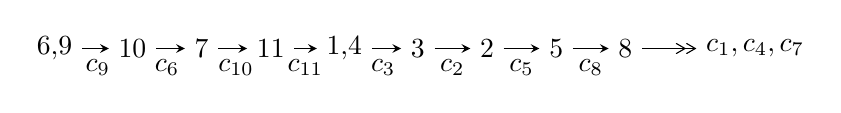
\begin{tikzpicture}[x=25pt, y=7pt]
	% node
	\node (A0) at (-1/8, 0) {6,9};
	\node (A1) at (1, 0) {10};
	\node (A2) at (2, 0) {7};
	\node (A3) at (3, 0) {11};
	\node (A4) at (65/16, 0) {1,4};
	\node (A5) at (41/8, 0) {3};
	\node (A6) at (49/8, 0) {2};
	\node (A7) at (57/8, 0) {5};
	\node (A8) at (65/8, 0) {8};
	\node (C1) at (1/2, -1) {$c_{9}$};
	\node (C2) at (3/2, -1) {$c_{6}$};
	\node (C3) at (5/2, -1) {$c_{10}$};
	\node (C4) at (7/2, -1) {$c_{11}$};
	\node (C5) at (37/8, -1) {$c_{3}$};
	\node (C6) at (45/8, -1) {$c_{2}$};
	\node (C7) at (53/8, -1) {$c_{5}$};
	\node (C8) at (61/8, -1) {$c_{8}$};
	\node (A9) at (10, 0) {$c_{1},c_{4},c_{7}$};

	% edge
	\draw[->,>=stealth]	
	(A0) edge (A1) (A1) edge (A2) (A2) edge (A3) (A3) edge (A4) (A4) edge (A5) (A5) edge (A6) (A6) edge (A7) (A7) edge (A8) ;
	\draw[->>,>={angle 60}]	
	(A8) edge (A9);
\end{tikzpicture} \\ 

\end{tabular} \\

\footnotetext{
The image of knot diagram is generated by the software ``\textbf{Draw programme}" developed by Andrew Bartholomew(\url{http://www.layer8.co.uk/maths/draw/index.htm\#Running-draw}), where we modified some parts for our purpose(\url{https://github.com/CATsTAILs/LinksPainter}).
}\phantom \\ \newline 
\centering \textbf{Ideals for irreducible components\footnotemark of $X_{\text{par}}$} 
 
\begin{align*}
I^u_{1}&=\langle 
- u^{15}- u^{14}+6 u^{13}+4 u^{12}-15 u^{11}-3 u^{10}+19 u^9-7 u^8-10 u^7+12 u^6-2 u^5-3 u^4+4 u^3-2 u^2+b+1,\\
\phantom{I^u_{1}}&\phantom{= \langle  }u^{15}+u^{14}-5 u^{13}-4 u^{12}+9 u^{11}+4 u^{10}-6 u^9+2 u^8- u^7-4 u^6+4 u^5-4 u^3+2 a+u-1,\\
\phantom{I^u_{1}}&\phantom{= \langle  }u^{16}+3 u^{15}+\cdots-3 u-2\rangle \\
I^u_{2}&=\langle 
-4 u^8 a+6 u^8+\cdots-3 a+4,\\
\phantom{I^u_{2}}&\phantom{= \langle  }-2 u^8 a+8 u^6 a+2 u^7+2 u^5 a+u^6-9 u^4 a-7 u^5-6 u^3 a-5 u^4+u^2 a+6 u^3+a^2+4 a u+7 u^2- a+2 u-2,\\
\phantom{I^u_{2}}&\phantom{= \langle  }u^9- u^8-4 u^7+3 u^6+5 u^5- u^4-2 u^3-2 u^2+u-1\rangle \\
I^u_{3}&=\langle 
u^5-2 u^3+b+u,\;u^5-3 u^3- u^2+a+2 u+1,\;u^6-3 u^4+2 u^2+1\rangle \\
\\
\end{align*}
\raggedright * 3 irreducible components of $\dim_{\mathbb{C}}=0$, with total 40 representations.\\
\footnotetext{All coefficients of polynomials are rational numbers. But the coefficients are sometimes approximated in decimal forms when there is not enough margin.}
\newpage
\renewcommand{\arraystretch}{1}
\centering \section*{I. $I^u_{1}= \langle - u^{15}- u^{14}+\cdots+b+1,\;u^{15}+u^{14}+\cdots+2 a-1,\;u^{16}+3 u^{15}+\cdots-3 u-2 \rangle$}
\flushleft \textbf{(i) Arc colorings}\\
\begin{tabular}{m{7pt} m{180pt} m{7pt} m{180pt} }
\flushright $a_{6}=$&$\begin{pmatrix}0\\u\end{pmatrix}$ \\
\flushright $a_{9}=$&$\begin{pmatrix}1\\0\end{pmatrix}$ \\
\flushright $a_{10}=$&$\begin{pmatrix}1\\- u^2\end{pmatrix}$ \\
\flushright $a_{7}=$&$\begin{pmatrix}u\\- u^3+u\end{pmatrix}$ \\
\flushright $a_{11}=$&$\begin{pmatrix}- u^2+1\\u^4-2 u^2\end{pmatrix}$ \\
\flushright $a_{1}=$&$\begin{pmatrix}- u^4+u^2+1\\u^4-2 u^2\end{pmatrix}$ \\
\flushright $a_{4}=$&$\begin{pmatrix}-\frac{1}{2} u^{15}-\frac{1}{2} u^{14}+\cdots-\frac{1}{2} u+\frac{1}{2}\\u^{15}+u^{14}+\cdots+2 u^2-1\end{pmatrix}$ \\
\flushright $a_{3}=$&$\begin{pmatrix}-\frac{3}{2} u^{15}-\frac{3}{2} u^{14}+\cdots-\frac{1}{2} u+\frac{3}{2}\\u^{15}+u^{14}+\cdots+2 u^2-1\end{pmatrix}$ \\
\flushright $a_{2}=$&$\begin{pmatrix}\frac{1}{2} u^{15}+\frac{1}{2} u^{14}+\cdots-\frac{1}{2} u+\frac{1}{2}\\- u^{15}- u^{14}+\cdots+u+1\end{pmatrix}$ \\
\flushright $a_{5}=$&$\begin{pmatrix}- u^5+2 u^3- u\\u^7-3 u^5+2 u^3+u\end{pmatrix}$ \\
\flushright $a_{8}=$&$\begin{pmatrix}\frac{3}{2} u^{15}+\frac{5}{2} u^{14}+\cdots-\frac{5}{2} u-\frac{3}{2}\\- u^{15}-2 u^{14}+\cdots-2 u^2+1\end{pmatrix}$\\ \flushright $a_{8}=$&$\begin{pmatrix}\frac{3}{2} u^{15}+\frac{5}{2} u^{14}+\cdots-\frac{5}{2} u-\frac{3}{2}\\- u^{15}-2 u^{14}+\cdots-2 u^2+1\end{pmatrix}$\\&\end{tabular}
\flushleft \textbf{(ii) Obstruction class $= -1$}\\~\\
\flushleft \textbf{(iii) Cusp Shapes $= 4 u^{15}+6 u^{14}-20 u^{13}-22 u^{12}+42 u^{11}+12 u^{10}-44 u^9+42 u^8+4 u^7-54 u^6+40 u^5-6 u^4-28 u^3+20 u^2-12 u+6$}\\~\\
\newpage\renewcommand{\arraystretch}{1}
\flushleft \textbf{(iv) u-Polynomials at the component}\newline \\
\begin{tabular}{m{50pt}|m{274pt}}
Crossings & \hspace{64pt}u-Polynomials at each crossing \\
\hline $$\begin{aligned}c_{1},c_{3},c_{4}\\c_{7},c_{8}\end{aligned}$$&$\begin{aligned}
&u^{16}+2 u^{14}+\cdots+2 u-1
\end{aligned}$\\
\hline $$\begin{aligned}c_{2}\end{aligned}$$&$\begin{aligned}
&u^{16}+4 u^{15}+\cdots-14 u^2+1
\end{aligned}$\\
\hline $$\begin{aligned}c_{5}\end{aligned}$$&$\begin{aligned}
&u^{16}+9 u^{15}+\cdots+31 u+22
\end{aligned}$\\
\hline $$\begin{aligned}c_{6},c_{9},c_{10}\end{aligned}$$&$\begin{aligned}
&u^{16}-3 u^{15}+\cdots+3 u-2
\end{aligned}$\\
\hline $$\begin{aligned}c_{11}\end{aligned}$$&$\begin{aligned}
&u^{16}-3 u^{15}+\cdots-41 u-8
\end{aligned}$\\
\hline
\end{tabular}\\~\\
\newpage\renewcommand{\arraystretch}{1}
\flushleft \textbf{(v) Riley Polynomials at the component}\newline \\
\begin{tabular}{m{50pt}|m{274pt}}
Crossings & \hspace{64pt}Riley Polynomials at each crossing \\
\hline $$\begin{aligned}c_{1},c_{3},c_{4}\\c_{7},c_{8}\end{aligned}$$&$\begin{aligned}
&y^{16}+4 y^{15}+\cdots-14 y^2+1
\end{aligned}$\\
\hline $$\begin{aligned}c_{2}\end{aligned}$$&$\begin{aligned}
&y^{16}+24 y^{15}+\cdots-28 y+1
\end{aligned}$\\
\hline $$\begin{aligned}c_{5}\end{aligned}$$&$\begin{aligned}
&y^{16}-3 y^{15}+\cdots-3557 y+484
\end{aligned}$\\
\hline $$\begin{aligned}c_{6},c_{9},c_{10}\end{aligned}$$&$\begin{aligned}
&y^{16}-15 y^{15}+\cdots-21 y+4
\end{aligned}$\\
\hline $$\begin{aligned}c_{11}\end{aligned}$$&$\begin{aligned}
&y^{16}+9 y^{15}+\cdots-6561 y+64
\end{aligned}$\\
\hline
\end{tabular}\\~\\
\newpage\flushleft \textbf{(vi) Complex Volumes and Cusp Shapes}
$$\begin{array}{c|c|c}  
\text{Solutions to }I^u_{1}& \I (\text{vol} + \sqrt{-1}CS) & \text{Cusp shape}\\
 \hline 
\begin{aligned}
u &= \phantom{-}0.608375 + 0.583971 I \\
a &= \phantom{-}0.147239 - 0.217444 I \\
b &= -0.826528 + 0.979522 I\end{aligned}
 & \phantom{-}3.36394 - 4.13872 I & \phantom{-}7.73528 + 1.97260 I \\ \hline\begin{aligned}
u &= \phantom{-}0.608375 - 0.583971 I \\
a &= \phantom{-}0.147239 + 0.217444 I \\
b &= -0.826528 - 0.979522 I\end{aligned}
 & \phantom{-}3.36394 + 4.13872 I & \phantom{-}7.73528 - 1.97260 I \\ \hline\begin{aligned}
u &= \phantom{-}0.395219 + 0.742683 I \\
a &= -1.25592 + 1.19798 I \\
b &= \phantom{-}0.797243 + 1.086110 I\end{aligned}
 & \phantom{-}2.59863 + 8.63192 I & \phantom{-}5.90792 - 7.27043 I \\ \hline\begin{aligned}
u &= \phantom{-}0.395219 - 0.742683 I \\
a &= -1.25592 - 1.19798 I \\
b &= \phantom{-}0.797243 - 1.086110 I\end{aligned}
 & \phantom{-}2.59863 - 8.63192 I & \phantom{-}5.90792 + 7.27043 I \\ \hline\begin{aligned}
u &= \phantom{-}1.216880 + 0.292072 I \\
a &= \phantom{-}0.840694 - 0.714472 I \\
b &= -0.494247 - 0.784033 I\end{aligned}
 & \phantom{-}0.99780 + 5.12268 I & \phantom{-}7.85223 - 7.82309 I \\ \hline\begin{aligned}
u &= \phantom{-}1.216880 - 0.292072 I \\
a &= \phantom{-}0.840694 + 0.714472 I \\
b &= -0.494247 + 0.784033 I\end{aligned}
 & \phantom{-}0.99780 - 5.12268 I & \phantom{-}7.85223 + 7.82309 I \\ \hline\begin{aligned}
u &= \phantom{-}0.012792 + 0.713635 I \\
a &= \phantom{-}0.244689 - 1.197750 I \\
b &= \phantom{-}0.379775 - 0.677130 I\end{aligned}
 & -2.70658 - 1.45405 I & \phantom{-}3.73411 + 4.71917 I \\ \hline\begin{aligned}
u &= \phantom{-}0.012792 - 0.713635 I \\
a &= \phantom{-}0.244689 + 1.197750 I \\
b &= \phantom{-}0.379775 + 0.677130 I\end{aligned}
 & -2.70658 + 1.45405 I & \phantom{-}3.73411 - 4.71917 I \\ \hline\begin{aligned}
u &= -1.271500 + 0.260922 I \\
a &= -0.319754 - 0.233539 I \\
b &= -0.232716 - 0.644221 I\end{aligned}
 & \phantom{-}1.24387 - 2.05073 I & \phantom{-}9.21244 - 1.11358 I \\ \hline\begin{aligned}
u &= -1.271500 - 0.260922 I \\
a &= -0.319754 + 0.233539 I \\
b &= -0.232716 + 0.644221 I\end{aligned}
 & \phantom{-}1.24387 + 2.05073 I & \phantom{-}9.21244 + 1.11358 I\\
 \hline 
 \end{array}$$\newpage$$\begin{array}{c|c|c}  
\text{Solutions to }I^u_{1}& \I (\text{vol} + \sqrt{-1}CS) & \text{Cusp shape}\\
 \hline 
\begin{aligned}
u &= \phantom{-}1.43214\phantom{ +0.000000I} \\
a &= -1.38066\phantom{ +0.000000I} \\
b &= \phantom{-}0.888414\phantom{ +0.000000I}\end{aligned}
 & \phantom{-}6.54271\phantom{ +0.000000I} & \phantom{-}14.4520\phantom{ +0.000000I} \\ \hline\begin{aligned}
u &= -1.47068 + 0.28044 I \\
a &= \phantom{-}2.09438 + 0.18309 I \\
b &= -0.82217 + 1.15830 I\end{aligned}
 & \phantom{-}8.6109 - 12.3641 I & \phantom{-}9.35094 + 7.14528 I \\ \hline\begin{aligned}
u &= -1.47068 - 0.28044 I \\
a &= \phantom{-}2.09438 - 0.18309 I \\
b &= -0.82217 - 1.15830 I\end{aligned}
 & \phantom{-}8.6109 + 12.3641 I & \phantom{-}9.35094 - 7.14528 I \\ \hline\begin{aligned}
u &= -1.50706 + 0.17257 I \\
a &= -1.11020 - 1.03847 I \\
b &= \phantom{-}0.966111 + 0.941274 I\end{aligned}
 & \phantom{-}10.25570 + 1.47993 I & \phantom{-}11.45831 - 1.74331 I \\ \hline\begin{aligned}
u &= -1.50706 - 0.17257 I \\
a &= -1.11020 + 1.03847 I \\
b &= \phantom{-}0.966111 - 0.941274 I\end{aligned}
 & \phantom{-}10.25570 - 1.47993 I & \phantom{-}11.45831 + 1.74331 I \\ \hline\begin{aligned}
u &= -0.400197\phantom{ +0.000000I} \\
a &= \phantom{-}0.598381\phantom{ +0.000000I} \\
b &= -0.423356\phantom{ +0.000000I}\end{aligned}
 & \phantom{-}0.656537\phantom{ +0.000000I} & \phantom{-}15.0460\phantom{ +0.000000I}\\
 \hline 
 \end{array}$$\newpage\newpage\renewcommand{\arraystretch}{1}
\centering \section*{II. $I^u_{2}= \langle -4 u^8 a+6 u^8+\cdots-3 a+4,\;-2 u^8 a+2 u^7+\cdots- a-2,\;u^9- u^8+\cdots+u-1 \rangle$}
\flushleft \textbf{(i) Arc colorings}\\
\begin{tabular}{m{7pt} m{180pt} m{7pt} m{180pt} }
\flushright $a_{6}=$&$\begin{pmatrix}0\\u\end{pmatrix}$ \\
\flushright $a_{9}=$&$\begin{pmatrix}1\\0\end{pmatrix}$ \\
\flushright $a_{10}=$&$\begin{pmatrix}1\\- u^2\end{pmatrix}$ \\
\flushright $a_{7}=$&$\begin{pmatrix}u\\- u^3+u\end{pmatrix}$ \\
\flushright $a_{11}=$&$\begin{pmatrix}- u^2+1\\u^4-2 u^2\end{pmatrix}$ \\
\flushright $a_{1}=$&$\begin{pmatrix}- u^4+u^2+1\\u^4-2 u^2\end{pmatrix}$ \\
\flushright $a_{4}=$&$\begin{pmatrix}a\\4 u^8 a-6 u^8+\cdots+3 a-4\end{pmatrix}$ \\
\flushright $a_{3}=$&$\begin{pmatrix}-4 u^8 a+6 u^8+\cdots-2 a+4\\4 u^8 a-6 u^8+\cdots+3 a-4\end{pmatrix}$ \\
\flushright $a_{2}=$&$\begin{pmatrix}-3 u^8 a+6 u^8+\cdots-2 a+5\\5 u^8 a-8 u^8+\cdots+4 a-6\end{pmatrix}$ \\
\flushright $a_{5}=$&$\begin{pmatrix}- u^5+2 u^3- u\\u^7-3 u^5+2 u^3+u\end{pmatrix}$ \\
\flushright $a_{8}=$&$\begin{pmatrix}6 u^8 a-9 u^8+\cdots+4 a-7\\-2 u^8 a+3 u^8+\cdots-2 a+2\end{pmatrix}$\\ \flushright $a_{8}=$&$\begin{pmatrix}6 u^8 a-9 u^8+\cdots+4 a-7\\-2 u^8 a+3 u^8+\cdots-2 a+2\end{pmatrix}$\\&\end{tabular}
\flushleft \textbf{(ii) Obstruction class $= -1$}\\~\\
\flushleft \textbf{(iii) Cusp Shapes $= -4 u^6+12 u^4+4 u^3-8 u^2-8 u+6$}\\~\\
\newpage\renewcommand{\arraystretch}{1}
\flushleft \textbf{(iv) u-Polynomials at the component}\newline \\
\begin{tabular}{m{50pt}|m{274pt}}
Crossings & \hspace{64pt}u-Polynomials at each crossing \\
\hline $$\begin{aligned}c_{1},c_{3},c_{4}\\c_{7},c_{8}\end{aligned}$$&$\begin{aligned}
&u^{18}- u^{17}+\cdots-8 u+5
\end{aligned}$\\
\hline $$\begin{aligned}c_{2}\end{aligned}$$&$\begin{aligned}
&u^{18}+7 u^{17}+\cdots+136 u+25
\end{aligned}$\\
\hline $$\begin{aligned}c_{5}\end{aligned}$$&$\begin{aligned}
&(u^9-3 u^8+2 u^7+5 u^6- u^5-13 u^4+10 u^3+2 u^2+u-3)^2
\end{aligned}$\\
\hline $$\begin{aligned}c_{6},c_{9},c_{10}\end{aligned}$$&$\begin{aligned}
&(u^9+u^8-4 u^7-3 u^6+5 u^5+u^4-2 u^3+2 u^2+u+1)^2
\end{aligned}$\\
\hline $$\begin{aligned}c_{11}\end{aligned}$$&$\begin{aligned}
&(u^9- u^8+6 u^7-5 u^6+11 u^5-7 u^4+6 u^3-2 u^2+u-1)^2
\end{aligned}$\\
\hline
\end{tabular}\\~\\
\newpage\renewcommand{\arraystretch}{1}
\flushleft \textbf{(v) Riley Polynomials at the component}\newline \\
\begin{tabular}{m{50pt}|m{274pt}}
Crossings & \hspace{64pt}Riley Polynomials at each crossing \\
\hline $$\begin{aligned}c_{1},c_{3},c_{4}\\c_{7},c_{8}\end{aligned}$$&$\begin{aligned}
&y^{18}+7 y^{17}+\cdots+136 y+25
\end{aligned}$\\
\hline $$\begin{aligned}c_{2}\end{aligned}$$&$\begin{aligned}
&y^{18}+7 y^{17}+\cdots+5004 y+625
\end{aligned}$\\
\hline $$\begin{aligned}c_{5}\end{aligned}$$&$\begin{aligned}
&(y^9-5 y^8+32 y^7-87 y^6+185 y^5-223 y^4+180 y^3-62 y^2+13 y-9)^{2}
\end{aligned}$\\
\hline $$\begin{aligned}c_{6},c_{9},c_{10}\end{aligned}$$&$\begin{aligned}
&(y^9-9 y^8+32 y^7-55 y^6+45 y^5-19 y^4+16 y^3-10 y^2-3 y-1)^2
\end{aligned}$\\
\hline $$\begin{aligned}c_{11}\end{aligned}$$&$\begin{aligned}
&(y^9+11 y^8+48 y^7+105 y^6+121 y^5+73 y^4+20 y^3-6 y^2-3 y-1)^2
\end{aligned}$\\
\hline
\end{tabular}\\~\\
\newpage\flushleft \textbf{(vi) Complex Volumes and Cusp Shapes}
$$\begin{array}{c|c|c}  
\text{Solutions to }I^u_{2}& \I (\text{vol} + \sqrt{-1}CS) & \text{Cusp shape}\\
 \hline 
\begin{aligned}
u &= -0.482242 + 0.666986 I \\
a &= \phantom{-}1.119660 + 0.834506 I \\
b &= -0.881705 + 0.851729 I\end{aligned}
 & \phantom{-}3.77376 - 2.21388 I & \phantom{-}8.24115 + 3.04598 I \\ \hline\begin{aligned}
u &= -0.482242 + 0.666986 I \\
a &= -0.009091 - 0.470353 I \\
b &= \phantom{-}0.937576 + 0.708026 I\end{aligned}
 & \phantom{-}3.77376 - 2.21388 I & \phantom{-}8.24115 + 3.04598 I \\ \hline\begin{aligned}
u &= -0.482242 - 0.666986 I \\
a &= \phantom{-}1.119660 - 0.834506 I \\
b &= -0.881705 - 0.851729 I\end{aligned}
 & \phantom{-}3.77376 + 2.21388 I & \phantom{-}8.24115 - 3.04598 I \\ \hline\begin{aligned}
u &= -0.482242 - 0.666986 I \\
a &= -0.009091 + 0.470353 I \\
b &= \phantom{-}0.937576 - 0.708026 I\end{aligned}
 & \phantom{-}3.77376 + 2.21388 I & \phantom{-}8.24115 - 3.04598 I \\ \hline\begin{aligned}
u &= \phantom{-}1.28056\phantom{ +0.000000I} \\
a &= \phantom{-}1.66854 + 0.09359 I \\
b &= -0.295309 + 1.123220 I\end{aligned}
 & -0.453072\phantom{ +0.000000I} & \phantom{-}5.66670\phantom{ +0.000000I} \\ \hline\begin{aligned}
u &= \phantom{-}1.28056\phantom{ +0.000000I} \\
a &= \phantom{-}1.66854 - 0.09359 I \\
b &= -0.295309 - 1.123220 I\end{aligned}
 & -0.453072\phantom{ +0.000000I} & \phantom{-}5.66670\phantom{ +0.000000I} \\ \hline\begin{aligned}
u &= -1.380230 + 0.162431 I \\
a &= -0.931046 + 0.163673 I \\
b &= \phantom{-}0.076831 - 1.264200 I\end{aligned}
 & \phantom{-}1.87293 - 3.41073 I & \phantom{-}9.88238 + 4.39642 I \\ \hline\begin{aligned}
u &= -1.380230 + 0.162431 I \\
a &= \phantom{-}1.54746 - 0.88517 I \\
b &= -0.505863 + 0.476260 I\end{aligned}
 & \phantom{-}1.87293 - 3.41073 I & \phantom{-}9.88238 + 4.39642 I \\ \hline\begin{aligned}
u &= -1.380230 - 0.162431 I \\
a &= -0.931046 - 0.163673 I \\
b &= \phantom{-}0.076831 + 1.264200 I\end{aligned}
 & \phantom{-}1.87293 + 3.41073 I & \phantom{-}9.88238 - 4.39642 I \\ \hline\begin{aligned}
u &= -1.380230 - 0.162431 I \\
a &= \phantom{-}1.54746 + 0.88517 I \\
b &= -0.505863 - 0.476260 I\end{aligned}
 & \phantom{-}1.87293 + 3.41073 I & \phantom{-}9.88238 - 4.39642 I\\
 \hline 
 \end{array}$$\newpage$$\begin{array}{c|c|c}  
\text{Solutions to }I^u_{2}& \I (\text{vol} + \sqrt{-1}CS) & \text{Cusp shape}\\
 \hline 
\begin{aligned}
u &= \phantom{-}0.230908 + 0.456719 I \\
a &= -1.90677 - 0.85951 I \\
b &= \phantom{-}0.257033 + 0.703723 I\end{aligned}
 & -3.25448 + 1.10969 I & \phantom{-}4.55374 - 6.23947 I \\ \hline\begin{aligned}
u &= \phantom{-}0.230908 + 0.456719 I \\
a &= \phantom{-}0.96790 - 1.89385 I \\
b &= \phantom{-}0.033137 - 1.191070 I\end{aligned}
 & -3.25448 + 1.10969 I & \phantom{-}4.55374 - 6.23947 I \\ \hline\begin{aligned}
u &= \phantom{-}0.230908 - 0.456719 I \\
a &= -1.90677 + 0.85951 I \\
b &= \phantom{-}0.257033 - 0.703723 I\end{aligned}
 & -3.25448 - 1.10969 I & \phantom{-}4.55374 + 6.23947 I \\ \hline\begin{aligned}
u &= \phantom{-}0.230908 - 0.456719 I \\
a &= \phantom{-}0.96790 + 1.89385 I \\
b &= \phantom{-}0.033137 + 1.191070 I\end{aligned}
 & -3.25448 - 1.10969 I & \phantom{-}4.55374 + 6.23947 I \\ \hline\begin{aligned}
u &= \phantom{-}1.49128 + 0.23430 I \\
a &= \phantom{-}1.01299 - 1.10233 I \\
b &= -1.067290 + 0.668745 I\end{aligned}
 & \phantom{-}10.17130 + 5.50049 I & \phantom{-}11.48937 - 2.97298 I \\ \hline\begin{aligned}
u &= \phantom{-}1.49128 + 0.23430 I \\
a &= -1.96964 - 0.01296 I \\
b &= \phantom{-}0.945590 + 0.965095 I\end{aligned}
 & \phantom{-}10.17130 + 5.50049 I & \phantom{-}11.48937 - 2.97298 I \\ \hline\begin{aligned}
u &= \phantom{-}1.49128 - 0.23430 I \\
a &= \phantom{-}1.01299 + 1.10233 I \\
b &= -1.067290 - 0.668745 I\end{aligned}
 & \phantom{-}10.17130 - 5.50049 I & \phantom{-}11.48937 + 2.97298 I \\ \hline\begin{aligned}
u &= \phantom{-}1.49128 - 0.23430 I \\
a &= -1.96964 + 0.01296 I \\
b &= \phantom{-}0.945590 - 0.965095 I\end{aligned}
 & \phantom{-}10.17130 - 5.50049 I & \phantom{-}11.48937 + 2.97298 I\\
 \hline 
 \end{array}$$\newpage\newpage\renewcommand{\arraystretch}{1}
\centering \section*{III. $I^u_{3}= \langle u^5-2 u^3+b+u,\;u^5-3 u^3- u^2+a+2 u+1,\;u^6-3 u^4+2 u^2+1 \rangle$}
\flushleft \textbf{(i) Arc colorings}\\
\begin{tabular}{m{7pt} m{180pt} m{7pt} m{180pt} }
\flushright $a_{6}=$&$\begin{pmatrix}0\\u\end{pmatrix}$ \\
\flushright $a_{9}=$&$\begin{pmatrix}1\\0\end{pmatrix}$ \\
\flushright $a_{10}=$&$\begin{pmatrix}1\\- u^2\end{pmatrix}$ \\
\flushright $a_{7}=$&$\begin{pmatrix}u\\- u^3+u\end{pmatrix}$ \\
\flushright $a_{11}=$&$\begin{pmatrix}- u^2+1\\u^4-2 u^2\end{pmatrix}$ \\
\flushright $a_{1}=$&$\begin{pmatrix}- u^4+u^2+1\\u^4-2 u^2\end{pmatrix}$ \\
\flushright $a_{4}=$&$\begin{pmatrix}- u^5+3 u^3+u^2-2 u-1\\- u^5+2 u^3- u\end{pmatrix}$ \\
\flushright $a_{3}=$&$\begin{pmatrix}u^3+u^2- u-1\\- u^5+2 u^3- u\end{pmatrix}$ \\
\flushright $a_{2}=$&$\begin{pmatrix}- u^4+u^3+2 u^2- u\\- u^5+u^4+2 u^3-2 u^2- u\end{pmatrix}$ \\
\flushright $a_{5}=$&$\begin{pmatrix}- u^5+2 u^3- u\\0\end{pmatrix}$ \\
\flushright $a_{8}=$&$\begin{pmatrix}- u^4- u^3+2 u^2+2 u\\-1\end{pmatrix}$\\ \flushright $a_{8}=$&$\begin{pmatrix}- u^4- u^3+2 u^2+2 u\\-1\end{pmatrix}$\\&\end{tabular}
\flushleft \textbf{(ii) Obstruction class $= 1$}\\~\\
\flushleft \textbf{(iii) Cusp Shapes $= -4 u^4+8 u^2$}\\~\\
\newpage\renewcommand{\arraystretch}{1}
\flushleft \textbf{(iv) u-Polynomials at the component}\newline \\
\begin{tabular}{m{50pt}|m{274pt}}
Crossings & \hspace{64pt}u-Polynomials at each crossing \\
\hline $$\begin{aligned}c_{1},c_{3},c_{4}\\c_{7},c_{8}\end{aligned}$$&$\begin{aligned}
&(u^2+1)^3
\end{aligned}$\\
\hline $$\begin{aligned}c_{2}\end{aligned}$$&$\begin{aligned}
&(u+1)^6
\end{aligned}$\\
\hline $$\begin{aligned}c_{5}\end{aligned}$$&$\begin{aligned}
&u^6+u^4+2 u^2+1
\end{aligned}$\\
\hline $$\begin{aligned}c_{6},c_{9},c_{10}\end{aligned}$$&$\begin{aligned}
&u^6-3 u^4+2 u^2+1
\end{aligned}$\\
\hline $$\begin{aligned}c_{11}\end{aligned}$$&$\begin{aligned}
&(u^3- u^2+1)^2
\end{aligned}$\\
\hline
\end{tabular}\\~\\
\newpage\renewcommand{\arraystretch}{1}
\flushleft \textbf{(v) Riley Polynomials at the component}\newline \\
\begin{tabular}{m{50pt}|m{274pt}}
Crossings & \hspace{64pt}Riley Polynomials at each crossing \\
\hline $$\begin{aligned}c_{1},c_{3},c_{4}\\c_{7},c_{8}\end{aligned}$$&$\begin{aligned}
&(y+1)^6
\end{aligned}$\\
\hline $$\begin{aligned}c_{2}\end{aligned}$$&$\begin{aligned}
&(y-1)^6
\end{aligned}$\\
\hline $$\begin{aligned}c_{5}\end{aligned}$$&$\begin{aligned}
&(y^3+y^2+2 y+1)^2
\end{aligned}$\\
\hline $$\begin{aligned}c_{6},c_{9},c_{10}\end{aligned}$$&$\begin{aligned}
&(y^3-3 y^2+2 y+1)^2
\end{aligned}$\\
\hline $$\begin{aligned}c_{11}\end{aligned}$$&$\begin{aligned}
&(y^3- y^2+2 y-1)^2
\end{aligned}$\\
\hline
\end{tabular}\\~\\
\newpage\flushleft \textbf{(vi) Complex Volumes and Cusp Shapes}
$$\begin{array}{c|c|c}  
\text{Solutions to }I^u_{3}& \I (\text{vol} + \sqrt{-1}CS) & \text{Cusp shape}\\
 \hline 
\begin{aligned}
u &= \phantom{-}1.307140 + 0.215080 I \\
a &= \phantom{-}1.40722 + 0.43972 I \\
b &= \phantom{-0.000000 } -1.000000 I\end{aligned}
 & -0.26574 + 2.82812 I & \phantom{-}3.50976 - 2.97945 I \\ \hline\begin{aligned}
u &= \phantom{-}1.307140 - 0.215080 I \\
a &= \phantom{-}1.40722 - 0.43972 I \\
b &= \phantom{-0.000000 -}1.000000 I\end{aligned}
 & -0.26574 - 2.82812 I & \phantom{-}3.50976 + 2.97945 I \\ \hline\begin{aligned}
u &= -1.307140 + 0.215080 I \\
a &= -0.082503 - 0.684841 I \\
b &= \phantom{-0.000000 } -1.000000 I\end{aligned}
 & -0.26574 - 2.82812 I & \phantom{-}3.50976 + 2.97945 I \\ \hline\begin{aligned}
u &= -1.307140 - 0.215080 I \\
a &= -0.082503 + 0.684841 I \\
b &= \phantom{-0.000000 -}1.000000 I\end{aligned}
 & -0.26574 + 2.82812 I & \phantom{-}3.50976 - 2.97945 I \\ \hline\begin{aligned}
u &= \phantom{-0.000000 -}0.569840 I \\
a &= -1.32472 - 1.75488 I \\
b &= \phantom{-0.000000 } -1.000000 I\end{aligned}
 & -4.40332\phantom{ +0.000000I} & -3.01950\phantom{ +0.000000I} \\ \hline\begin{aligned}
u &= \phantom{-0.000000 } -0.569840 I \\
a &= -1.32472 + 1.75488 I \\
b &= \phantom{-0.000000 -}1.000000 I\end{aligned}
 & -4.40332\phantom{ +0.000000I} & -3.01950\phantom{ +0.000000I}\\
 \hline 
 \end{array}$$\newpage
\newpage\renewcommand{\arraystretch}{1}
\centering \section*{ IV. u-Polynomials}
\begin{tabular}{m{50pt}|m{274pt}}
Crossings & \hspace{64pt}u-Polynomials at each crossing \\
\hline $$\begin{aligned}c_{1},c_{3},c_{4}\\c_{7},c_{8}\end{aligned}$$&$\begin{aligned}
&((u^2+1)^3)(u^{16}+2 u^{14}+\cdots+2 u-1)(u^{18}- u^{17}+\cdots-8 u+5)
\end{aligned}$\\
\hline $$\begin{aligned}c_{2}\end{aligned}$$&$\begin{aligned}
&((u+1)^6)(u^{16}+4 u^{15}+\cdots-14 u^2+1)(u^{18}+7 u^{17}+\cdots+136 u+25)
\end{aligned}$\\
\hline $$\begin{aligned}c_{5}\end{aligned}$$&$\begin{aligned}
&(u^6+u^4+2 u^2+1)\\
&\cdot(u^9-3 u^8+2 u^7+5 u^6- u^5-13 u^4+10 u^3+2 u^2+u-3)^2\\
&\cdot(u^{16}+9 u^{15}+\cdots+31 u+22)
\end{aligned}$\\
\hline $$\begin{aligned}c_{6},c_{9},c_{10}\end{aligned}$$&$\begin{aligned}
&(u^6-3 u^4+2 u^2+1)\\
&\cdot(u^9+u^8-4 u^7-3 u^6+5 u^5+u^4-2 u^3+2 u^2+u+1)^2\\
&\cdot(u^{16}-3 u^{15}+\cdots+3 u-2)
\end{aligned}$\\
\hline $$\begin{aligned}c_{11}\end{aligned}$$&$\begin{aligned}
&((u^3- u^2+1)^2)(u^9- u^8+\cdots+u-1)^{2}\\
&\cdot(u^{16}-3 u^{15}+\cdots-41 u-8)
\end{aligned}$\\
\hline
\end{tabular}\newpage\renewcommand{\arraystretch}{1}
\centering \section*{ V. Riley Polynomials}
\begin{tabular}{m{50pt}|m{274pt}}
Crossings & \hspace{64pt}Riley Polynomials at each crossing \\
\hline $$\begin{aligned}c_{1},c_{3},c_{4}\\c_{7},c_{8}\end{aligned}$$&$\begin{aligned}
&((y+1)^6)(y^{16}+4 y^{15}+\cdots-14 y^2+1)(y^{18}+7 y^{17}+\cdots+136 y+25)
\end{aligned}$\\
\hline $$\begin{aligned}c_{2}\end{aligned}$$&$\begin{aligned}
&((y-1)^6)(y^{16}+24 y^{15}+\cdots-28 y+1)(y^{18}+7 y^{17}+\cdots+5004 y+625)
\end{aligned}$\\
\hline $$\begin{aligned}c_{5}\end{aligned}$$&$\begin{aligned}
&(y^3+y^2+2 y+1)^2\\
&\cdot(y^9-5 y^8+32 y^7-87 y^6+185 y^5-223 y^4+180 y^3-62 y^2+13 y-9)^{2}\\
&\cdot(y^{16}-3 y^{15}+\cdots-3557 y+484)
\end{aligned}$\\
\hline $$\begin{aligned}c_{6},c_{9},c_{10}\end{aligned}$$&$\begin{aligned}
&(y^3-3 y^2+2 y+1)^2\\
&\cdot(y^9-9 y^8+32 y^7-55 y^6+45 y^5-19 y^4+16 y^3-10 y^2-3 y-1)^2\\
&\cdot(y^{16}-15 y^{15}+\cdots-21 y+4)
\end{aligned}$\\
\hline $$\begin{aligned}c_{11}\end{aligned}$$&$\begin{aligned}
&(y^3- y^2+2 y-1)^2\\
&\cdot(y^9+11 y^8+48 y^7+105 y^6+121 y^5+73 y^4+20 y^3-6 y^2-3 y-1)^2\\
&\cdot(y^{16}+9 y^{15}+\cdots-6561 y+64)
\end{aligned}$\\
\hline
\end{tabular}
\vskip 2pc
\end{document}